\part{Course introduction}
\section{Introduction}
\subsection*{General}

\begin{frame}
 \frametitle{Numerical Methods}
 \renewcommand{\thefootnote}{$\star$} 
  {\LARGE ``Simulation and mathematical modeling will power the twenty-first century the way steam powered the nineteenth.''\\
   {\vspace{1em}\hspace{2em} --- W.H. Press\footnote{Author of Numerical recipes, in ``The Nature of Mathematical Modeling'' by Neil Gershenfeld }}} \\
  \vspace{-1cm}
  \flushright\tikz{\node[opacity=0.4] at (4cm,-0.5) {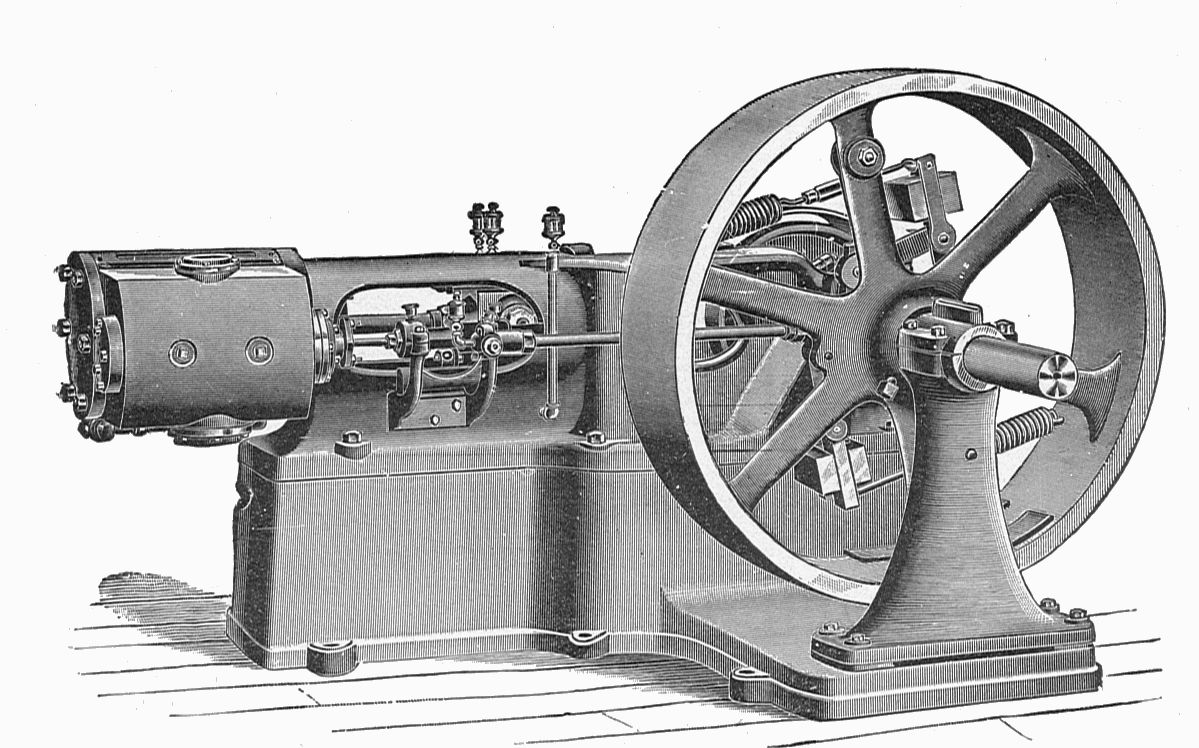
\includegraphics[width=0.5\textwidth]{sengine.jpg}};}
\end{frame}

\begin{frame}
 \frametitle{Ptolemy and the almagest}
 \begin{columns}
   \column{0.5\textwidth}\centering
     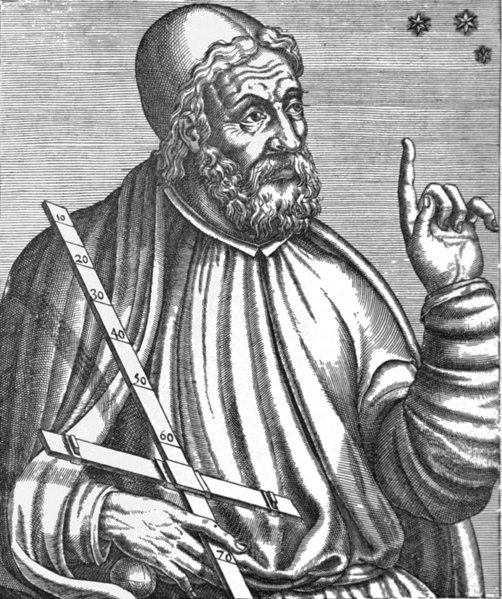
\includegraphics[height=0.7\columnwidth]{Ptolemy.png}
   \column{0.5\textwidth}\centering
     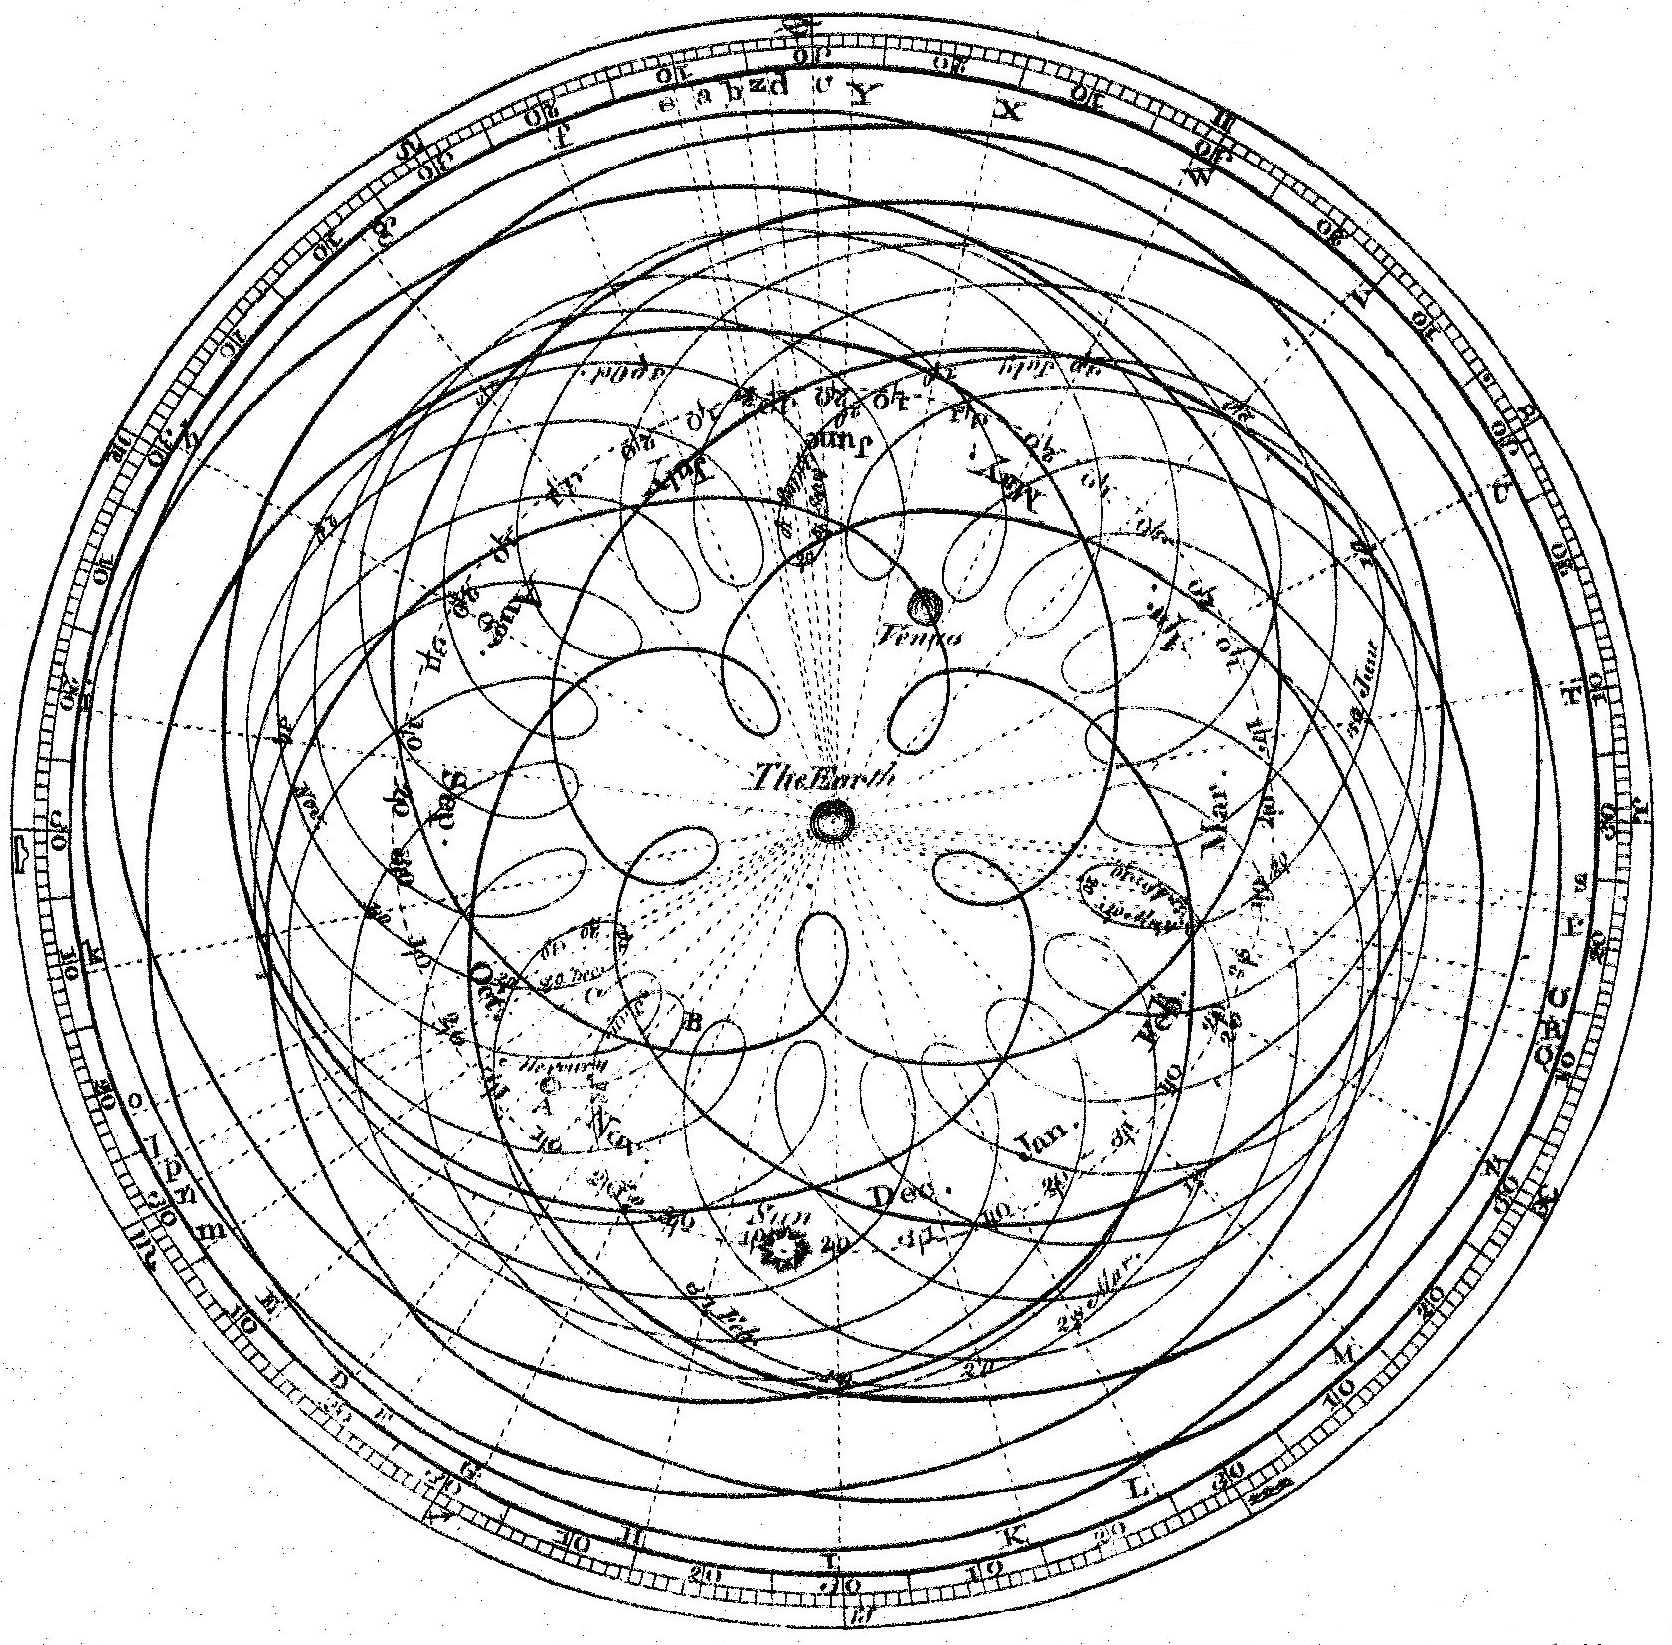
\includegraphics[width=0.8\columnwidth]{Cassini_apparent.png}   
 \end{columns} \vspace{1em}
 \tikz{\node[emphblock,text width=\textwidth]{
   ${\sim}150$ AD. Development of numerical approximations to describe the motions of the heavenly bodies with accuracy matching reality sufficiently.};}
\end{frame}

\begin{frame}
 \frametitle{Numerical Methods}
 \begin{itemize}
  \item Numerical analysis is concerned with obtaining approximate solutions to problems while maintaining reasonable bounds of error...
  \item ...because it is often impossible to obtain exact answers ...
  \item Numerical analysis makes use of algorithms to
approximate solutions
 \end{itemize}
\end{frame}

\begin{frame}
 \frametitle{Used in many fields... Including Chemical Engineering}
  \begin{itemize}
	  \item Description of reactors and separators (dynamic and steady state)
		\item Computational fluid dynamics
		\item Thermodynamic equations of state
		\item Optimizing process performance
		\item Design and synthesis of processes
		\item Regression of data, e.g. isotherms, kinetics, ...
 \end{itemize}
\end{frame}

\section{About this course}
\subsection{About}
\begin{frame}
 \frametitle{Course Schedule}
 \centering
 \begin{tabular}{ccll}
 \hline
 Lecture & Date & Topic & Teacher \\ 
 \hline
 1  & 09/11/2020 & Programming and algorithms (1)       & IR \\ 
 2  & 12/11/2020 & Programming and algorithms (2)       & IR \\ 
 3  & 16/11/2020 & Numerical errors                     & IR \\ 
 4  & 19/11/2020 & Interpolation, integration           & IR \\ 
 5  & 23/12/2020 & Curve fitting, regression            & IR \\ 
 6  & 26/11/2020 & Linear eqns: direct methods          & IR\\ 
 7  & 30/11/2020 & Linear eqns: iterative methods       & IR \\ 
 8  & 03/11/2020 & Non-linear equations (1)             & MSA \\ 
 9  & 07/12/2020 & Non-linear equations (2)             & MSA\\ 
 10 & 20/12/2020 & Ordinary differential equations (1)  & MSA \\
 11 & 14/12/2020 & Ordinary differential equations (2)  & MSA \\ 
 12 & 17/12/2020 & Partial differential equations       & MSA \\ 
 \hline
 \end{tabular} 
\end{frame}

\begin{frame}
 \frametitle{Course Objectives}
 \begin{itemize}
  \item Gain experience with programming basics and algorithm design
  \item Acquire knowledge of and experience with various techniques for the numerical solution of systems of linear and non-linear algebraic and differential equations, as well as data analysis and optimization.
  \item Being able to solve various numerical problems using Matlab or Excel. 
 \end{itemize}
\end{frame}

\begin{frame}
 \frametitle{Prerequisites}
  The following courses should give you enough background knowledge to follow this course comfortably:
 \begin{itemize}
   \item Calculus
   \item Linear Algebra
   \item Some basic MATLAB experience
     \begin{itemize}
       \item We will cover some aspects on MATLAB programming in the first lectures. Detailed documents and courses are provided on Canvas, for your own reference.
     \end{itemize}
    \end{itemize}
    You will definitely need a laptop with Matlab and Excel installed!
\end{frame}

\begin{frame}
 \frametitle{Course Materials}
 \begin{itemize}
  \item Lecture slides + lecture recordings
  \item MATLAB scripts
  \item Additional articles
  \item There are some useful books for those seeking more in-depth knowledge and alternative methods, not mandatory:
  \begin{itemize}
    \item Numerical recipes, W.H. Press et al.
    \item Numerical methods for chemical engineering, K.J. Beers
    \item Numerical methods for chemical engineers, A. Constantinides
    \item Essential matlab-for engineers, B.D. Hahn
    \item Introduction to Numerical Methods and Matlab Programming for Engineers, T. Young and M.J. Mohlenkamp
  \end{itemize}
 \end{itemize}
  \tikz{\node[emphblock,text width=\textwidth]{
    Look on Canvas for the slides, exercises, scripts, assignments and additional documentation on MATLAB.
   };}
\end{frame}

\section{Assessments}
\subsection{Assessments}
\begin{frame}
 \frametitle{Assessment}
 \begin{block}{4 assignments}
  \begin{itemize}
    \item Each 15\% of the final result
    \item Done in groups of 2 persons, see Canvas$\,\to\,$People
    \item Short report (template provided, Overleaf and Canvas)
    \item Questions on the assignments should be asked in-class, not through private message/mail/etc.
  \end{itemize}   
 \end{block}
 \pause
 \begin{block}{Final exam}
  \begin{itemize}
    \item Practical and theoretical questions, covering \emph{all topics}
    \item Exam taken on your own computer (ANS with proctorio+Matlab), opt-out through on-campus exam with screen sharing, camera surveillance and invigilators.
    \item You can use the slides and Matlab documentation
    \item Sample exam will be released before Christmas
    \item Grade of the final exam needs to be at least a 5.0
  \end{itemize}   
 \end{block}
\end{frame}

\begin{frame}
\frametitle{Assignment grading: peer assessment \& feedback (1)}
\begin{itemize}
  \item Assignments are graded through supervised peer-assessment. After the deadline, each \emph{person} will grade 2 other assignments. Rubrics are available to maintain a consistent assessment among different groups. Criteria are:
    \begin{itemize}
      \item Functionality
      \item Code style
      \item Visualisation
      \item Analysis
    \end{itemize}
  \item The assessment should be done within 3 days using rubrics, additional feedback should be supplied to establish its validity. We will assess the quality of the feedback, and grade it by a multiplier (0.8-1.2).
  \item You can challenge one or more reviews by submitting a rebuttal; 

  \item The final grade will be the averaged grade from the remaining peer-assessments (group), multiplied by the peer-review quality (individual), with a max. of 10.
  \item When statistics are poor ($\leq 2$ reviews), the assignment will be graded by the instructor, which discards all remaining peer-reviews.
\end{itemize}
\end{frame}

\begin{frame}
\frametitle{Assignment grading: peer assessment \& feedback (2)}
\begin{itemize}
    \item Along with the rubrics, you will give each other specific comments for improvement: What are you impressed with; why did you score a certain criteria low; how to improve the code or  visuals, etc. Give at least 3 tips and 3 tops.
    \item Grades for an assignment are released only when proper assessment and feedback have been given.
    \item Rebuttals are turned in through an additional assignment. A rebuttal should convince us and provide evidence and in-depth argumentation why a particular review is flawed. We will evaluate the rebuttals and discard a peer-review if it is indeed disproportionate.
    \item We are getting help from student assistants to make the process go smoothly. I will show a possible solution after the deadline.
    \item Grading with rubrics: don't be afraid to use the full spectrum.
\end{itemize}

\end{frame}

\begin{frame}
  \frametitle{Peer assessment in the past}
  \begin{columns}
    \column{0.5\textwidth}\centering
      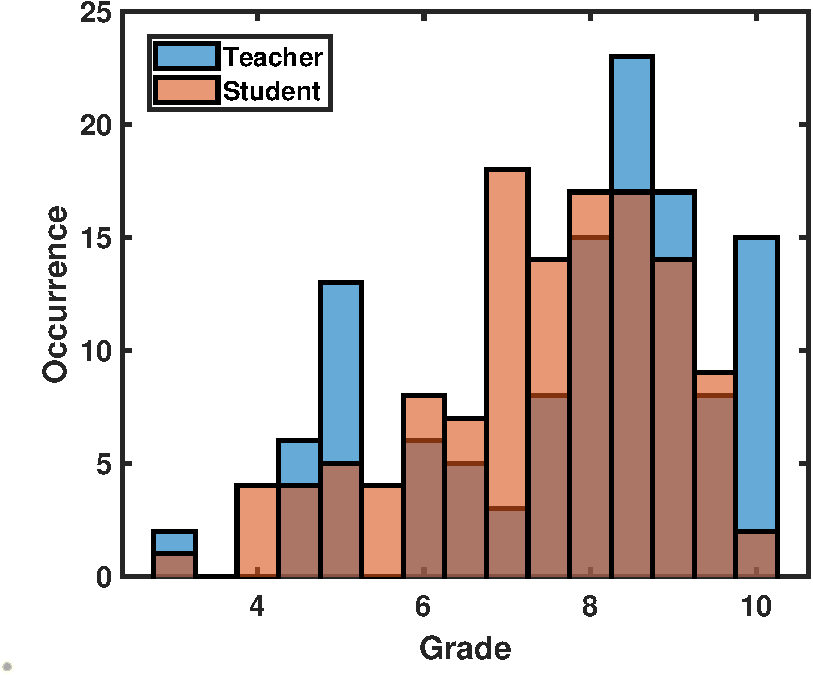
\includegraphics[height=0.8\columnwidth]{histogram-TS-crop}
    \column{0.5\textwidth}\centering
      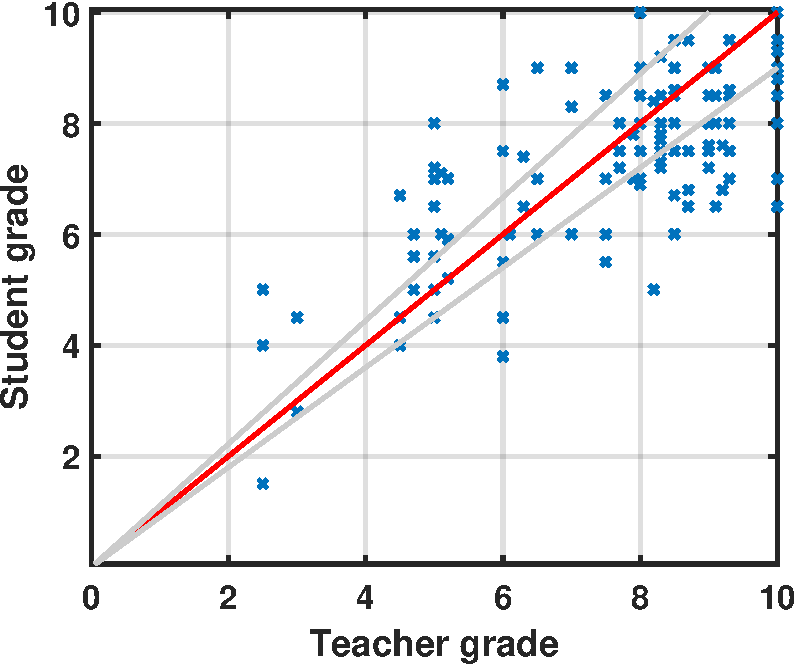
\includegraphics[width=0.8\columnwidth]{scatter}   
  \end{columns}
 \end{frame}

 \begin{frame}
  \frametitle{Peer assessment summary}
  Complete document can be read through Canvas, here's the summary:
  \begin{itemize}
    \item The assignment and report template are released along with the grading rubrics
    \item Canvas automatically performs a plagiarism check
    \item The lecturer will give a short overview of how the assignment could have been solved (point of reference)
    \item Students have 3 days for double-blind peer assessment
    \item Students have the opportunity to challenge their reviewers (rebuttal)
    \item Lecturers and TAs will check the review quality, as well as the reports that have very low or very high marks or large deviations among reviews coarsely. I will provide a full correction when no suitable peer-reviews have been done.
    \item If a student fails to produce a good, timely peer-review, their grade for the assignment will be marked NA.
  \end{itemize}
 \end{frame}
%
\begin{frame}
 \frametitle{Assignment handout and deadlines}
     Hand-in your assignments via Canvas
    \begin{itemize}
      \item Deadlines are given on Canvas as well
      \item Deliver the report in PDF format
      \item Send along the scripts + necessities in a .zip
      \item Use your student ID instead of your name for identification purposes
    \end{itemize}
\end{frame}


\section{Finally...}
\subsection{Information}
\begin{frame}
 \frametitle{Course Philosophy}
 \begin{itemize}
  \item This is a hard course! It will take a lot of hours, especially if you have no coding experience.
  \item We are here to help you. To have nice discussions, to show alternative ways, etc. Clarify language subtleties, or suggestions. Not to give away the answers.
  \item We encourage research and independent learning. It comes down to paying attention, repetition of the concepts, and practice practice practice! 
  \item We try to make the lectures interactive, working on examples and creating scripts as we go. It is advised that you work along with us to get the most out of this course!
  \item It is ok to discuss the general approach to solving the problem, or to get a hint, or several hints, if you get stuck while solving a problem, but work out the details of the solution in your own group.
  \item It is {\textbf{not ok}} to take someone else’s solution and simply copy their scripts, answers, etc.
  \item Take regular breaks! Better 6 times per hour a short break than 1 time per hour a long break. Use keyboard shortcuts, or a mouse if you must. Set up screen brightness to a pleasant value. Stretch.
 \end{itemize}
\end{frame}

\begin{frame}
 \frametitle{Contact information}
 \begin{block}{Ivo Roghair}
  \begin{itemize}
%    \item Contact via Canvas is preferred!
   \item E-mail: \href{mailto:i.roghair@tue.nl}{i.roghair@tue.nl}
   \item Office: STW 0.37
   \end{itemize} 
 \end{block}
 \vspace{1em}
  \begin{block}{Martin van Sint Annaland}
  \begin{itemize}
   \item E-mail: \href{mailto:m.v.sintannaland@tue.nl}{m.v.sintannaland@tue.nl}
   \item Office: STW 0.39 
   \end{itemize} 
 \end{block}
\end{frame}

% \begin{frame}
%  \frametitle{Some last remarks}
%   \begin{itemize}
%   \item Tell us if something is not clear.
%   \item We try to make the lectures interactive, working on examples and creating scripts as we go. It is advised that you work along with us to get the most out of this course!
%   \item The exercises are meant to provide a jump start towards the assignments.
%   \item We will always answer questions on the exercises. We may didactically answer questions on the assignments.
%   \item During the lectures/tutorials we first and foremost work on the exercises. If they are done, you can work on the assignment if you want.
%   \end{itemize} 
% \end{frame}

\begin{frame}
 \frametitle{Some Acknowledgements}
 \centering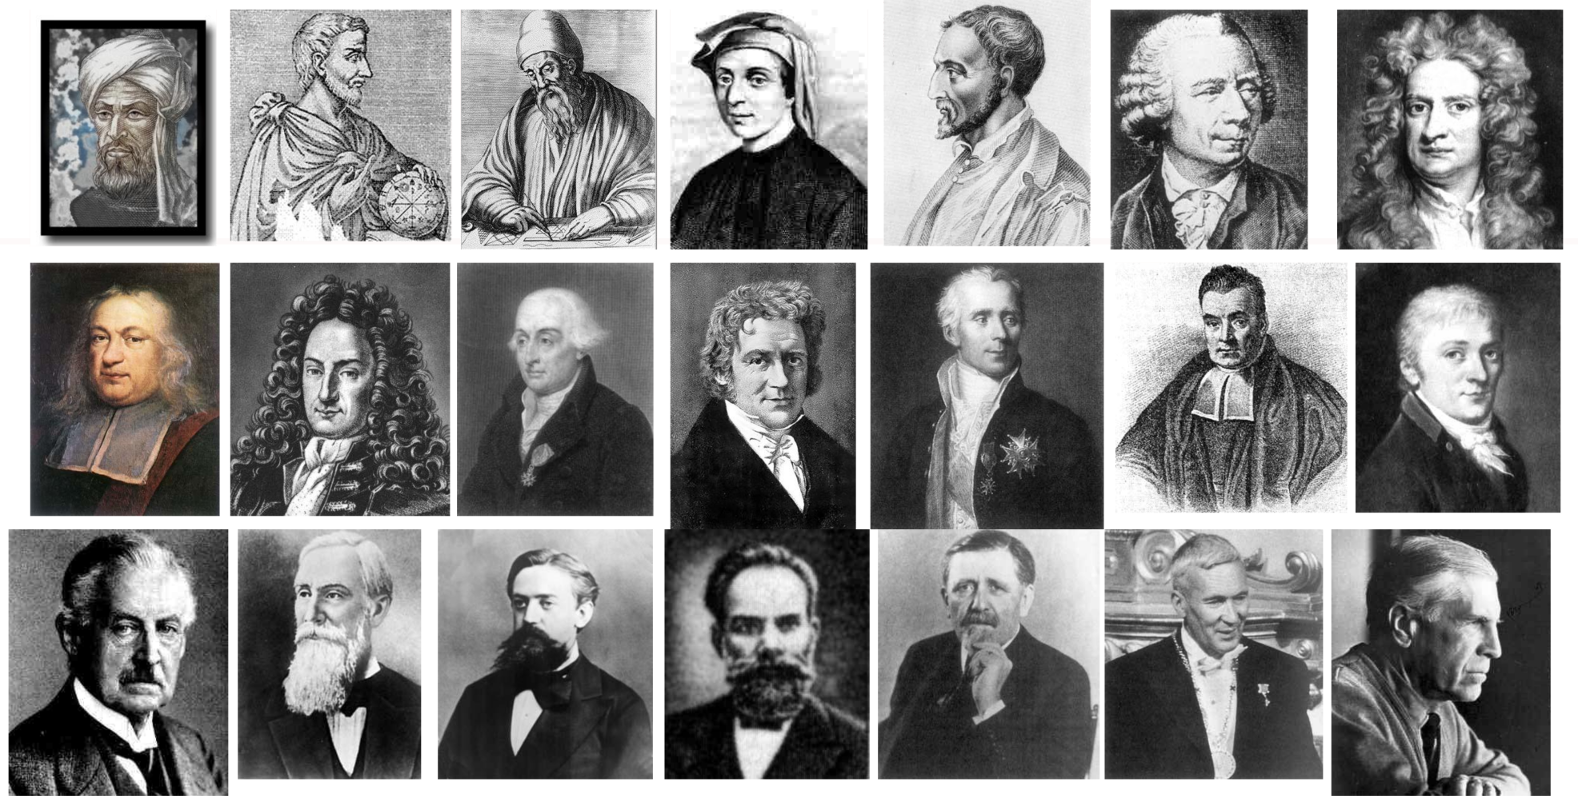
\includegraphics[width=\textwidth]{ack.png}
\end{frame}

\begin{frame}
 \frametitle{Some Real Acknowledgements}
 For inspiration, examples and exercises:
 \begin{itemize}
  \item To Roel Verstappen of Groningen University
  \item To Johan Hult of Cambridge University
  \item To Edwin Zondervan of Universit\"at Bremen
  \item To edX: MITx course  "Introduction to Computer Science and Programming Using Python"
 \end{itemize}
\end{frame}
% \end{document}


% References
% http://ocw.mit.edu/courses/electrical-engineering-and-computer-science/6-00sc-introduction-to-computer-science-and-programming-spring-2011/unit-1/lecture-1-introduction-to-6.00/
% http://www.greenteapress.com/thinkpython/html/thinkpython002.html
% https://www.youtube.com/channel/UCLMQ21H2ad95faYG3yGCwYA
%http://stackoverflow.com/questions/4227145/in-matlab-are-variables-really-double-precision-by-default
%http://www.exploringbinary.com/why-0-point-1-does-not-exist-in-floating-point/

